\section{Best Subset Selection}
\subsection{Theory}
The best subset selection is a selection method trying all outcomes with the different predictors ($p$) of a given dataset. Going through the subset selection stepwise:
\begin{enumerate}
	\item Start off with the null model ($M_0$). This model is a model without any predictors, and is used to calculate the sample mean. 
	\item Next step, for $k = 1, 2, \dots p$ fit the $( \begin{smallmatrix} p \\ k \end{smallmatrix} )$ with exactly $k$ predictors. Pick the best among the $( \begin{smallmatrix} p \\ k \end{smallmatrix} )$ models, and call this $M_k$, where best is defined as the smallest $RSS$ or highest $R^2$.
	\item Last step, select a single best model from among $M_0,\dots,M_p$ using cross-validated prediction error, $C_p$ (AIC), BIC, or adjusted $R^2$.
\end{enumerate}
 
Using the best subset selection is one of the better ways of deciding the most efficient predictors of a given dataset, however going through all outcomes this way, takes a lot of computation power. Using formula \ref{fo:BestSubsetCalculationAmounts}, the amount of computations can be calculated for each calculation of $M_k$. if all possibilities are tested, the amount of computations becomes $O(2^p)$.
\begin{align}\label{fo:BestSubsetCalculationAmounts}
	\begin{pmatrix}
		p \\ k
	\end{pmatrix}
	= \dfrac{p!}{k!(p-k)!}
\end{align}

The best subset selection method can also lead to overfitting and high variance of the coefficient estimates, which is unwanted in most cases. 

These two reasons make stepwise methods a very attractive alternative, to best subset selection. 

\subsection{Results}
\subsubsection*{LAB 6.5.1}%TODO Rewrite, remove "we"
In Lab 6.5.1, we look at baseball player data, and want to predict their salary on the basis of various statistics associated with their performance in the previous year. In this lab we start off by removing the data that insufficient data. Then because we are using python, we have to define some formulas to calculate the RSS and best subset selection algorithm, these have been found on another git repository\footnote{\cite{Xu2017}}.

The result of the subset selection on the data can be seen on Figure \ref{fig:bestSubsetSelection} with an RSS value on the graph on the left, and Adjusted $R^2$ on the graph on the right. Observe that the Adjusted $R^2$ graph starts to decay the higher the  amount of predictors, after approximately 10 predictors. Theory behind this in Section \ref{sc:estimatingTestError} Estimating Test Error Using Mallow's Cp, AIC, BIC and Adjusted R-squared, on page \pageref{sc:estimatingTestError}.

\begin{figure}[h]
	\centering
	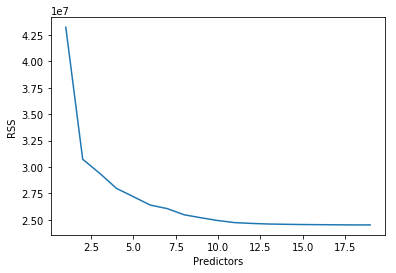
\includegraphics[scale=0.5]{subsetSelection/selectionMethods/fig/bestSubsetSelectionRSS.png}
	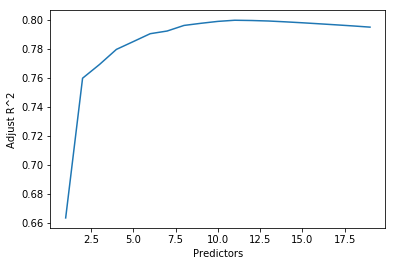
\includegraphics[scale=0.5]{subsetSelection/selectionMethods/fig/bestSubsetSelectionRsquared.png}
	\caption{Best Subset Selection predicting salary on baseball players.}
	\label{fig:bestSubsetSelection}
\end{figure}


\section{Forward/Backward Stepwise Selection}
\subsection{Theory}
Forward and backward stepwise selection are pretty similar, the difference is whether to start the model with no predictors (Forward) or to start the model with all predictors (Backward). These two methods are not guaranteed to yield the best model containing a subset of the $p$ predictors, unlike the best subset selection, but their computations are far more efficient than best subset selection.

\textbf{Forward stepwise selection}, begins with a model containing no predictors, and then stepwise adds predictors to the model, however for each step the variable that gives the greatest additional improvement the fit is added. This means that not every single combination of $k$ predictors are analyzed, instead only one additional predictor at $k$ step is added to the already decided $k-1$ predictors, from the steps beforehand. Going through the forward stepwise selection:
\begin{enumerate}
	\item Let $M_0$ denote the null model, which contains no predictors.
	\item For $k=0,\dots,p-1$:
	\begin{enumerate}
		\item Consider all $p-k$ models that augment the predictors in $M_k$ with one additional predictor.
		\item Choose the best among these $p-k$ models, and call it $M_{k+1}$. Here best is defined as having smallest RSS or highest $R^2$.
	\end{enumerate}
	\item Select a single best model from among $M_0,\dots,M_p$ using cross-validated prediction error, $C_p$ (AIC), BIC, or adjusted $R^2$. 
\end{enumerate}

The amount of computations is given by $1+p+(p-1)+\dots+(p-k)$. If all possibilities are tested, the amount of computations becomes $O(p^2)$. This is an advantage over the best subset selection with $O(2^p)$.

\textbf{Backward stepwise selection}, has a lot of similarities to the forward stepwise selection, just in reverse. Instead of starting with null model, this method start with the full least squares model containing all $p$ predictors. This backward stepwise selection have the same advantages as forward stepwise selection over the best subset selection. Going through the backward stepwise selection:

\begin{enumerate}
	\item Let $M_p$ denote the full least squares model, containing all $p$ predictors.
	\item For $k=p,p-1,\dots,1$:
	\begin{enumerate}
		\item Consider all $k$ models that contain all but one predictor in $M_k$, adding up to a total of $k-1$ predictors.
		\item Choose the best among these $k$ models, and call it $M_{k-1}$. Here best is defined as having smallest RSS or highest $R^2$.
	\end{enumerate}
	\item Select a single best model from among $M_0,\dots,M_p$ using cross-validated prediction error, $C_p$ (AIC), BIC, or adjusted $R^2$. 
\end{enumerate}

If all possibilities are tested, the amount of computations becomes $O(p^2)$, just like the forward stepwise selection method. This is an advantage over the best subset selection with $O(2^p)$.

\subsection{Results}
\subsubsection*{LAB 6.5.2}
In Lab 6.5.2, we continue to look at baseball players and try to predict their salary on the basis of various statistics associated with their performance in the previous year. We use the same procedure to prepare the data and once again define some functions to calculate RSS and use the forward and backward stepwise selection method.

After calculating forward and backward stepwise selection two methods give two different results. On Figure \ref{fig:forwardBackwardStepwiseSelectionRSS} the two methods have been illustrated and it is easy to see that the results are different even though they are closely related. Do we look at what the two different methods got as predictors at $k=3$ we see that forward stepwise selection chose the three predictors "Hits", "CRBI" and "Division\_W", where backward stepwise selection chose "Hits", "CRuns" and "PutOuts".

\begin{figure}[h]
	\centering
	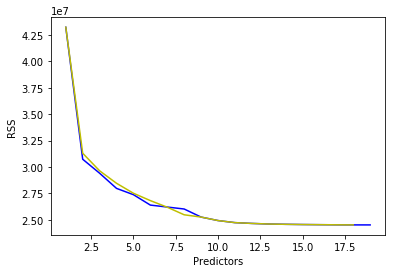
\includegraphics[scale=0.5]{subsetSelection/selectionMethods/fig/forwardBackwardStepwiseSelectionRSS.png}
	\caption{Forward and Backward Stepwise Selection predicting salary on baseball players. Forward is blue, Backward is yellow.}
	\label{fig:forwardBackwardStepwiseSelectionRSS}
\end{figure}

